\documentclass[a0,landscape]{a0poster}

\usepackage[paper=a0paper, landscape, margin=2cm]{geometry}

\usepackage{multicol} % This is so we can have multiple columns of text side-by-side
\columnsep=100pt % This is the amount of white space between the columns in the poster
\columnseprule=1pt

\usepackage{tikz}

\usepackage{sectsty}
\sectionfont{\huge\selectfont}

\usepackage[scaled]{helvet}
\renewcommand\familydefault{\sfdefault} 
\usepackage[T1]{fontenc}

\usepackage{graphicx} % Required for including images
\graphicspath{{figures/}} % Location of the graphics files
\usepackage{booktabs} % Top and bottom rules for table
\usepackage[font=small,labelfont=bf]{caption} % Required for specifying captions to tables and figures
\usepackage{amsfonts, amsmath, amsthm, amssymb} % For math fonts, symbols and environments
\usepackage{wrapfig} % Allows wrapping text around tables and figures

\usepackage{caption}
\captionsetup{margin=2cm,font=large,labelfont=bf}
\newenvironment{Figure}
  {\par\medskip\noindent\minipage{\linewidth}}
  {\endminipage\par\medskip}

%\usepackage{pgfplots}
%\usepackage{pgfplotstable}
%\pgfplotsset{compat=newest}
%\usepgfplotslibrary{external}
%\tikzexternalize

\begin{document}

\tikz[remember picture,overlay] \node[inner sep=0pt, anchor=north] at (current page.north){
\includegraphics[width=\paperwidth,height=12cm]{GreenBackground.pdf}};

\vspace{-1cm}
\begin{minipage}[t]{0.3\linewidth}
\vspace{0pt}

\includegraphics[width=0.9\textwidth]{UofALogo.pdf}
\end{minipage}
%
\begin{minipage}[t]{0.7\linewidth}
\vspace{0.75cm}
\color{white}
\veryHuge \textbf{\textsc{Redliner: An Activity Monitor for Manual Wheelchair Users}}\\[1cm]
\huge {Kenton Hamaluik, MSc, EIT\textsuperscript{1}, Zohreh Salimi, MSc\textsuperscript{1}, Martin Ferguson-Pell, PhD, C.Phys.\textsuperscript{1,2}}\\
\large \textsuperscript{1}Faculty of Rehabilitation Medicine,\ \textsuperscript{2}Peter Lougheed Leadership College\\
\end{minipage}

\vspace{4cm}

\begin{multicols*}{3}
\large

\section*{Background}
\begin{itemize}
    \item Wheelchair users have a strong need to monitor activity
        \begin{itemize}
            \item Manual wheelchair users are highly susceptible to repetitive stress injuries \cite{big}
            \item Propulsion forces over 80\% of maximum capacity result in damage \cite{small}
        \end{itemize}
    \item Typical existing activity monitors don't work with manual wheelchair users
    \item SmartWheels are the gold standard, but are an expensive clinical tool
        \begin{itemize}
            \item There is a need for an affordable consumer-grade tool for activity monitoring
        \end{itemize}
\end{itemize}

\section*{Objective}
The objective of this work was to create an inexpensive activity monitor for manual wheelchair users capable of measuring the following data:

\begin{itemize}
    \item Number of propulsion strokes
    \item Average travel velocity
    \item Amount of time spent active
    \item Estimated distance travelled
    \item Number of ``redline events''\textsuperscript{1}
\end{itemize}

\textsuperscript{1} \textit{redline events} are instances of when the user's propulsion force exceeds 80\% of the maximal propulsion force they can generate

\section*{Method}

\section*{Results}
As you can see in Figure \ref{fig:10pushgravel}, derp.

\begin{Figure}
    \centering
    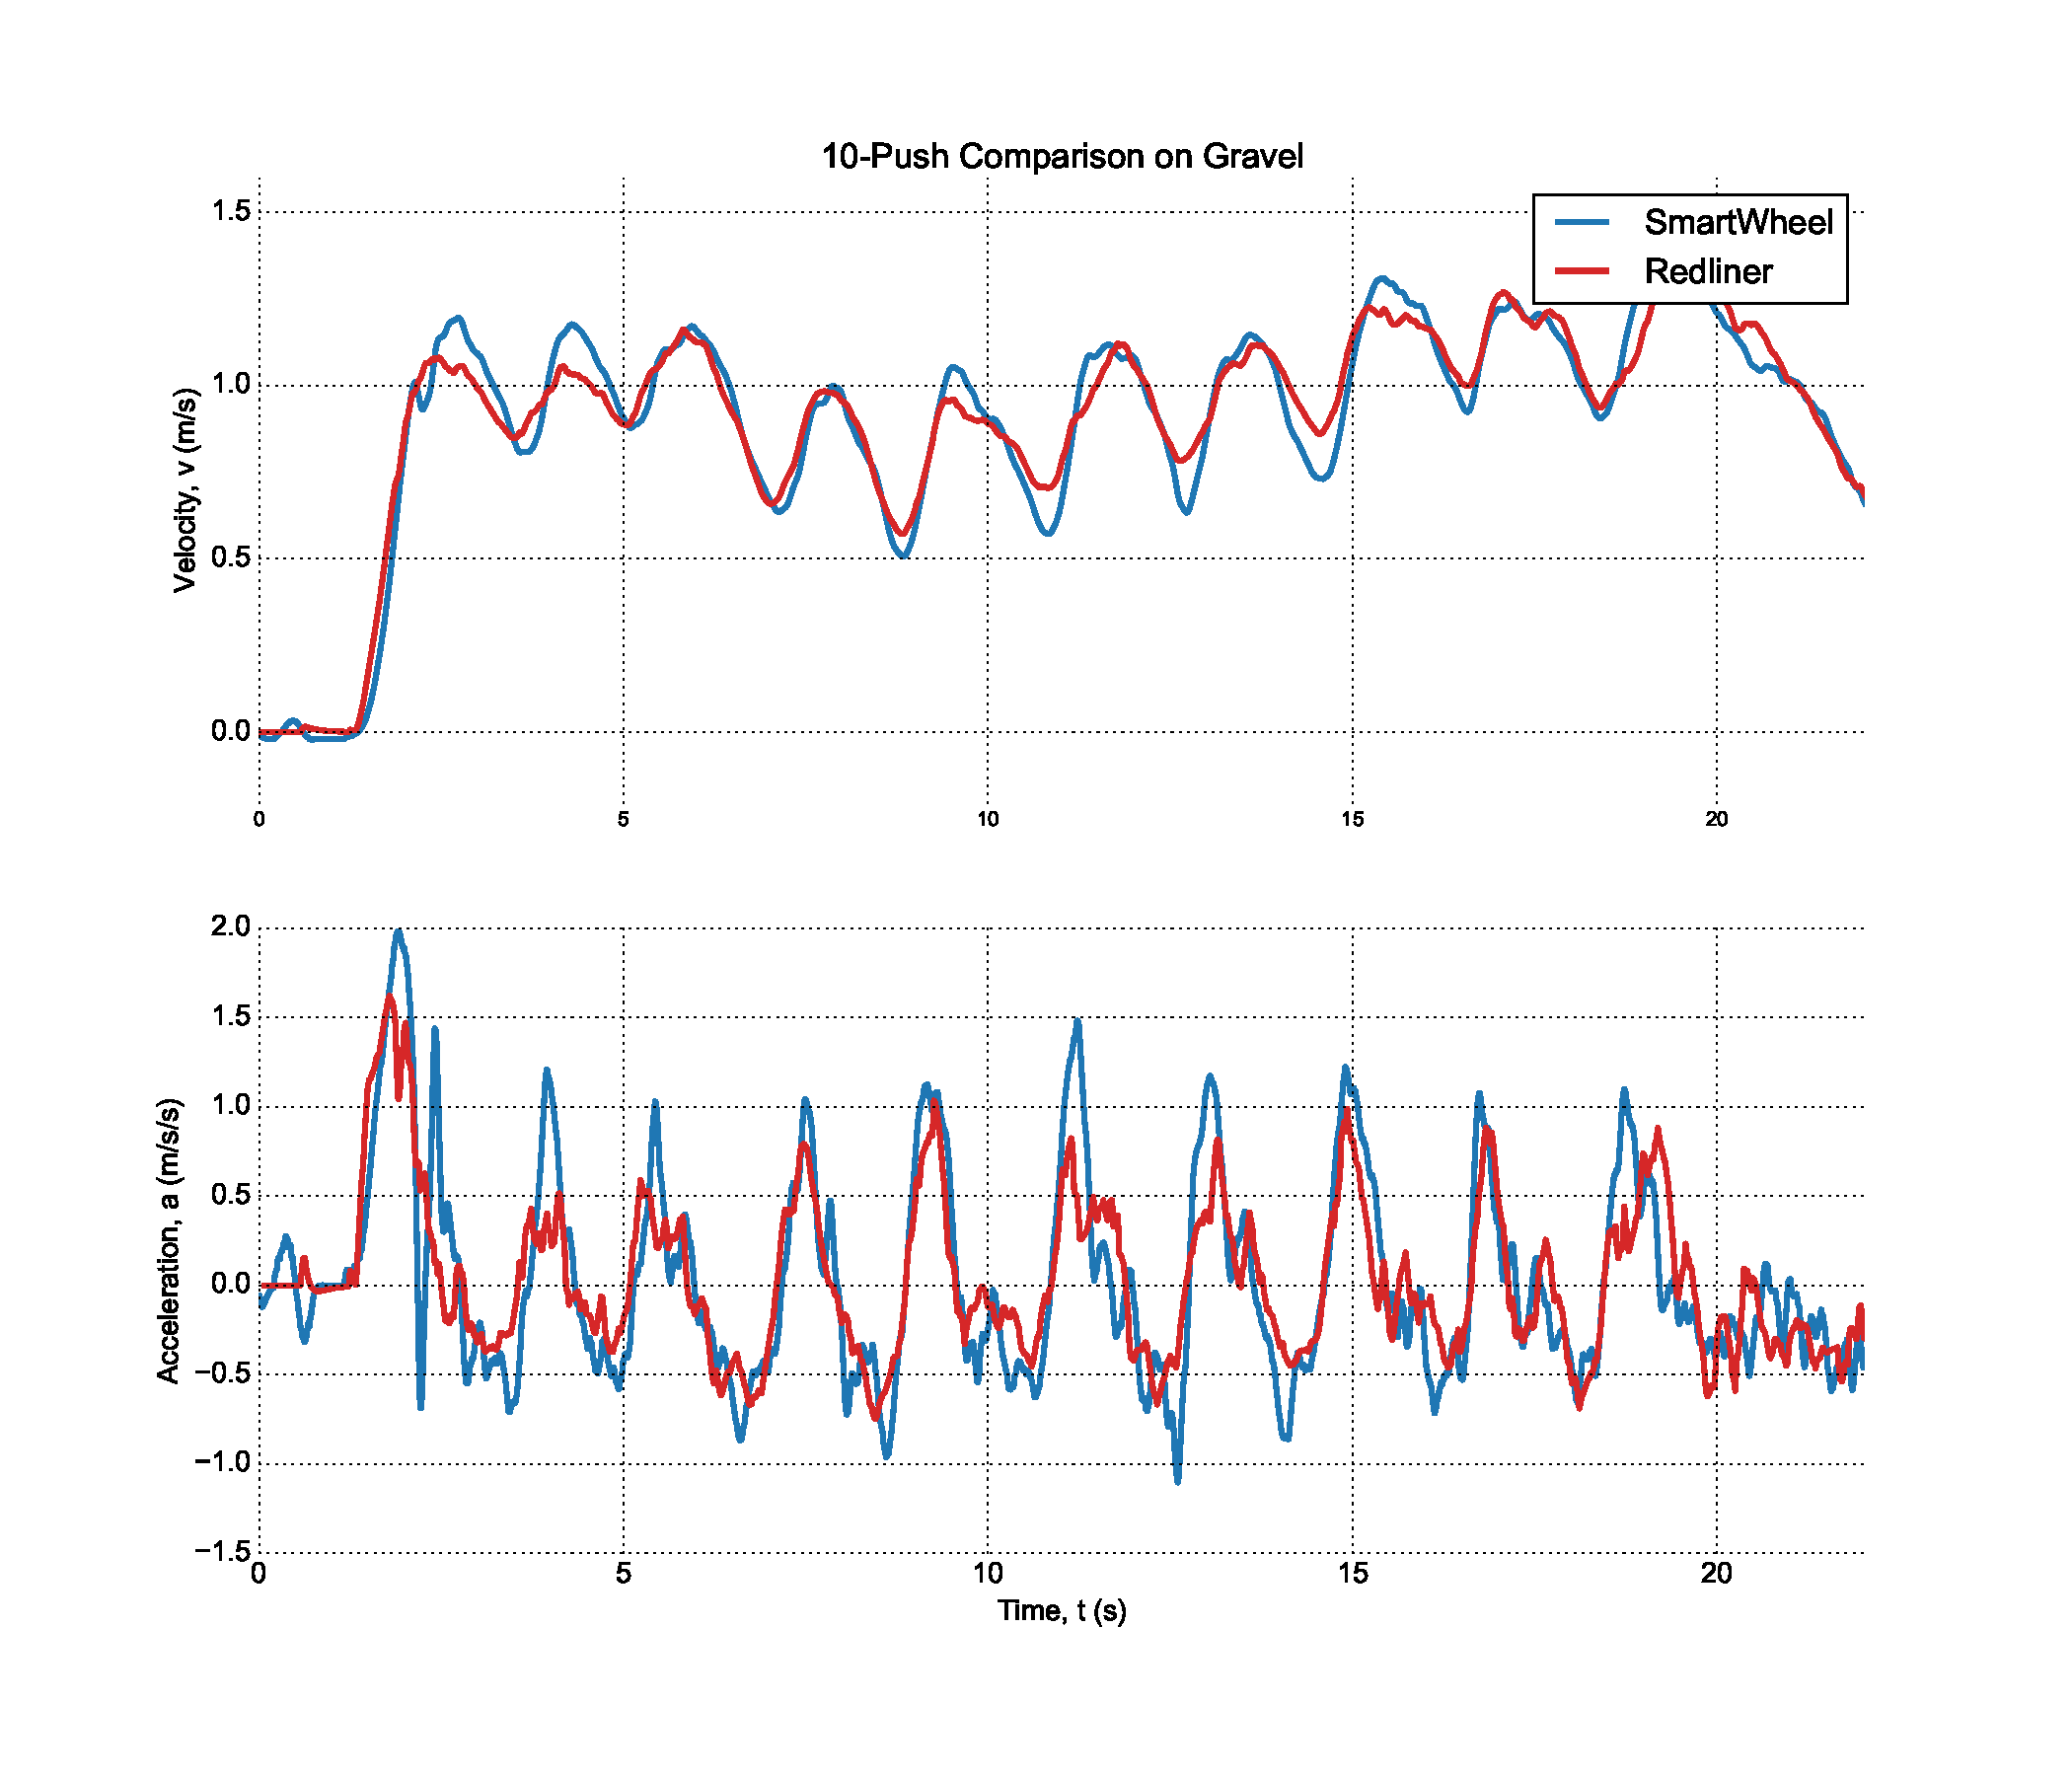
\includegraphics[width=\linewidth]{data/assets/test.pdf}
    \captionof{figure}{Velocity and acceleration traces for both Redliner and SmartWheel for 10 pushes on rough gravel. The traces are in close enough agreement to accurately count pushes and reasonably estimate exertion and distance travelled with Redliner---despite the excess noise caused by the rough terrain.}
    \label{fig:10pushgravel}
\end{Figure}

\section*{Conclusions}
\begin{itemize}
    \item Redliner is a new activity monitor for manual wheelchair users
    \item Redliner has been validated against expensive SmartWheel devices
    \item Redliner is moving forward as a commercial entity to produce and sell the devices
\end{itemize}

\nocite{*} % Print all references regardless of whether they were cited in the poster or not
\bibliographystyle{plain} % Plain referencing style
\bibliography{sources} % Use the example bibliography file sample.bib

\section*{Acknowledgements}
Funding for this work was provided for by the University of Alberta, Telus, the Government of Canada, and Redliner Inc.

\end{multicols*}
\end{document}
